\documentclass{article}

\usepackage{fullpage}
\usepackage{graphicx}


\title{Sesión 5: Caracterización de un filtro RCL}
\date{}
\author{Pablo Cuesta Sierra. Grupo 1201. Puesto 10.}



\begin{document}

\maketitle
\begin{center}
\section*{MONTAJE EXPERIMENTAL}
\end{center}
\textbf{Monte el circuito 1 con $R_1 = 4.7k\Omega$, $C_1 = 100nF$ y $L_1 = 10mH$. La señal de tensión
sinusoidal V1 se obtiene del terminal Output del generador de funciones, fijando inicialmente
una amplitud de 1V y variando su frecuencia. Con el cable BNC-banana conectaremos la señal
a la entrenadora.}\bigskip

\begin{center}
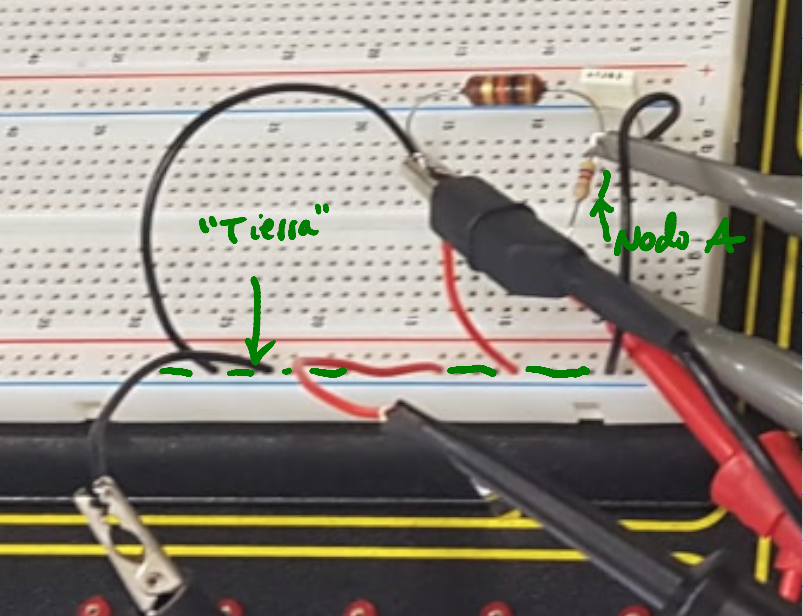
\includegraphics[scale=0.3]{circuito2}\\
Circuito montado en la entrenadora.
\end{center}

\textbf{Varíe la frecuencia del generador desde 50 Hz hasta 500 KHz logarítmicamente. Utilice
los dos canales del osciloscopio y mida la amplitud de V1 ($V_1$), la amplitud de la tensión entre
los nodos A y B ($V_{AB}$) y el desfase temporal de ambas señales para cada una de las frecuencias.
Calcule el cociente $A_v$ entre las amplitudes $V_AB$ y $V_1$ ($A_v=V_{AB}/V_1$) Finalmente, convierta
el desfase temporal a grados o radianes. Con esos datos se debería poder rellenar una tabla como
la siguiente:}

El cálculo de los ángulos de la fase en grados es de la siguiente forma:
$$\Phi (^o)=360^o\times \delta t \times f$$
\cleardoublepage

\begin{table}[!h]
\centering
\begin{tabular}{|r|r|r|r|r|l|}
\hline
\multicolumn{1}{|l|}{frecuencia(Hz)} & \multicolumn{1}{l|}{$V_1(V)$} & \multicolumn{1}{l|}{$V_{AB}(V)$} & \multicolumn{1}{l|}{$A_v$} & \multicolumn{1}{l|}{$\delta t(s)$} & $\Phi (^o)$                   \\ \hline
50                                   & 1                             & 0,0091                           & 0,0091                     & 0,00012                            & 2,16     \\ \hline
60                                   & 1,01                          & 0,0093                           & 0,009207920792             & 0,00013                            & 2,808    \\ \hline
80                                   & 1,02                          & 0,0094                           & 0,009215686275             & 0,00018                            & 5,184    \\ \hline
100                                  & 1,01                          & 0,0094                           & 0,009306930693             & 0,00022                            & 7,92     \\ \hline
300                                  & 1,02                          & 0,0102                           & 0,01                       & 0,00024                            & 25,92    \\ \hline
500                                  & 1,02                          & 0,0116                           & 0,01137254902              & 0,000212                           & 38,16    \\ \hline
700                                  & 1,02                          & 0,0136                           & 0,01333333333              & 0,000184                           & 46,368   \\ \hline
900                                  & 1,01                          & 0,016                            & 0,01584158416              & 0,000172                           & 55,728   \\ \hline
1000                                 & 1,01                          & 0,0173                           & 0,01712871287              & 0,00016                            & 57,6     \\ \hline
3000                                 & 1,03                          & 0,063                            & 0,06116504854              & 0,000063                           & 68,04    \\ \hline
4900                                 & 1,04                          & 0,318                            & 0,3057692308               & 0,0000148                          & 26,1072  \\ \hline
5000                                 & 1,04                          & 0,342                            & 0,3288461538               & 0,0000024                          & 4,32     \\ \hline
5100                                 & 1,04                          & 0,356                            & 0,3423076923               & -0,0000016                         & -2,9376  \\ \hline
5200                                 & 1,04                          & 0,354                            & 0,3403846154               & -0,0000056                         & -10,4832 \\ \hline
7000                                 & 1,04                          & 0,108                            & 0,1038461538               & -0,0000308                         & -77,616  \\ \hline
9000                                 & 1,04                          & 0,061                            & 0,05865384615              & -0,000026                          & -84,24   \\ \hline
10000                                & 1,04                          & 0,051                            & 0,04903846154              & -0,0000244                         & -87,84   \\ \hline
30000                                & 1,03                          & 0,0134                           & 0,01300970874              & -0,0000082                         & -88,56   \\ \hline
50000                                & 1,03                          & 0,0084                           & 0,008155339806             & -0,000005                          & -90      \\ \hline
70000                                & 1                             & 0,00525                          & 0,00525                    & -0,0000036                         & -90,72   \\ \hline
90000                                & 0,99                          & 0,00404                          & 0,004080808081             & -0,00000276                        & -89,424  \\ \hline
100000                               & 0,99                          & 0,00364                          & 0,003676767677             & -0,00000248                        & -89,28   \\ \hline
300000                               & 0,99                          & 0,00124                          & 0,001252525253             & -0,00000081                        & -87,48   \\ \hline
500000                               & 1                             & 0,00076                          & 0,00076                    & -0,00000042                        & -75,6    \\ \hline
\end{tabular}
\end{table}


Nota: Las últimas diferencias de fase son negativas, esto se debe a que se invertía el orden de las ondas, $V_1$ y $V_{AB}$. Esto sucede a partir de la frecuencia natural del circuito. Nótese que ha ido variando la amplitud de la onda proporcionada por el generador de funciones, aunque el valor que estaba establecido en este era de amplitud 1V, se ha tenido esto en cuenta al calcular la ganancia.


\begin{center}
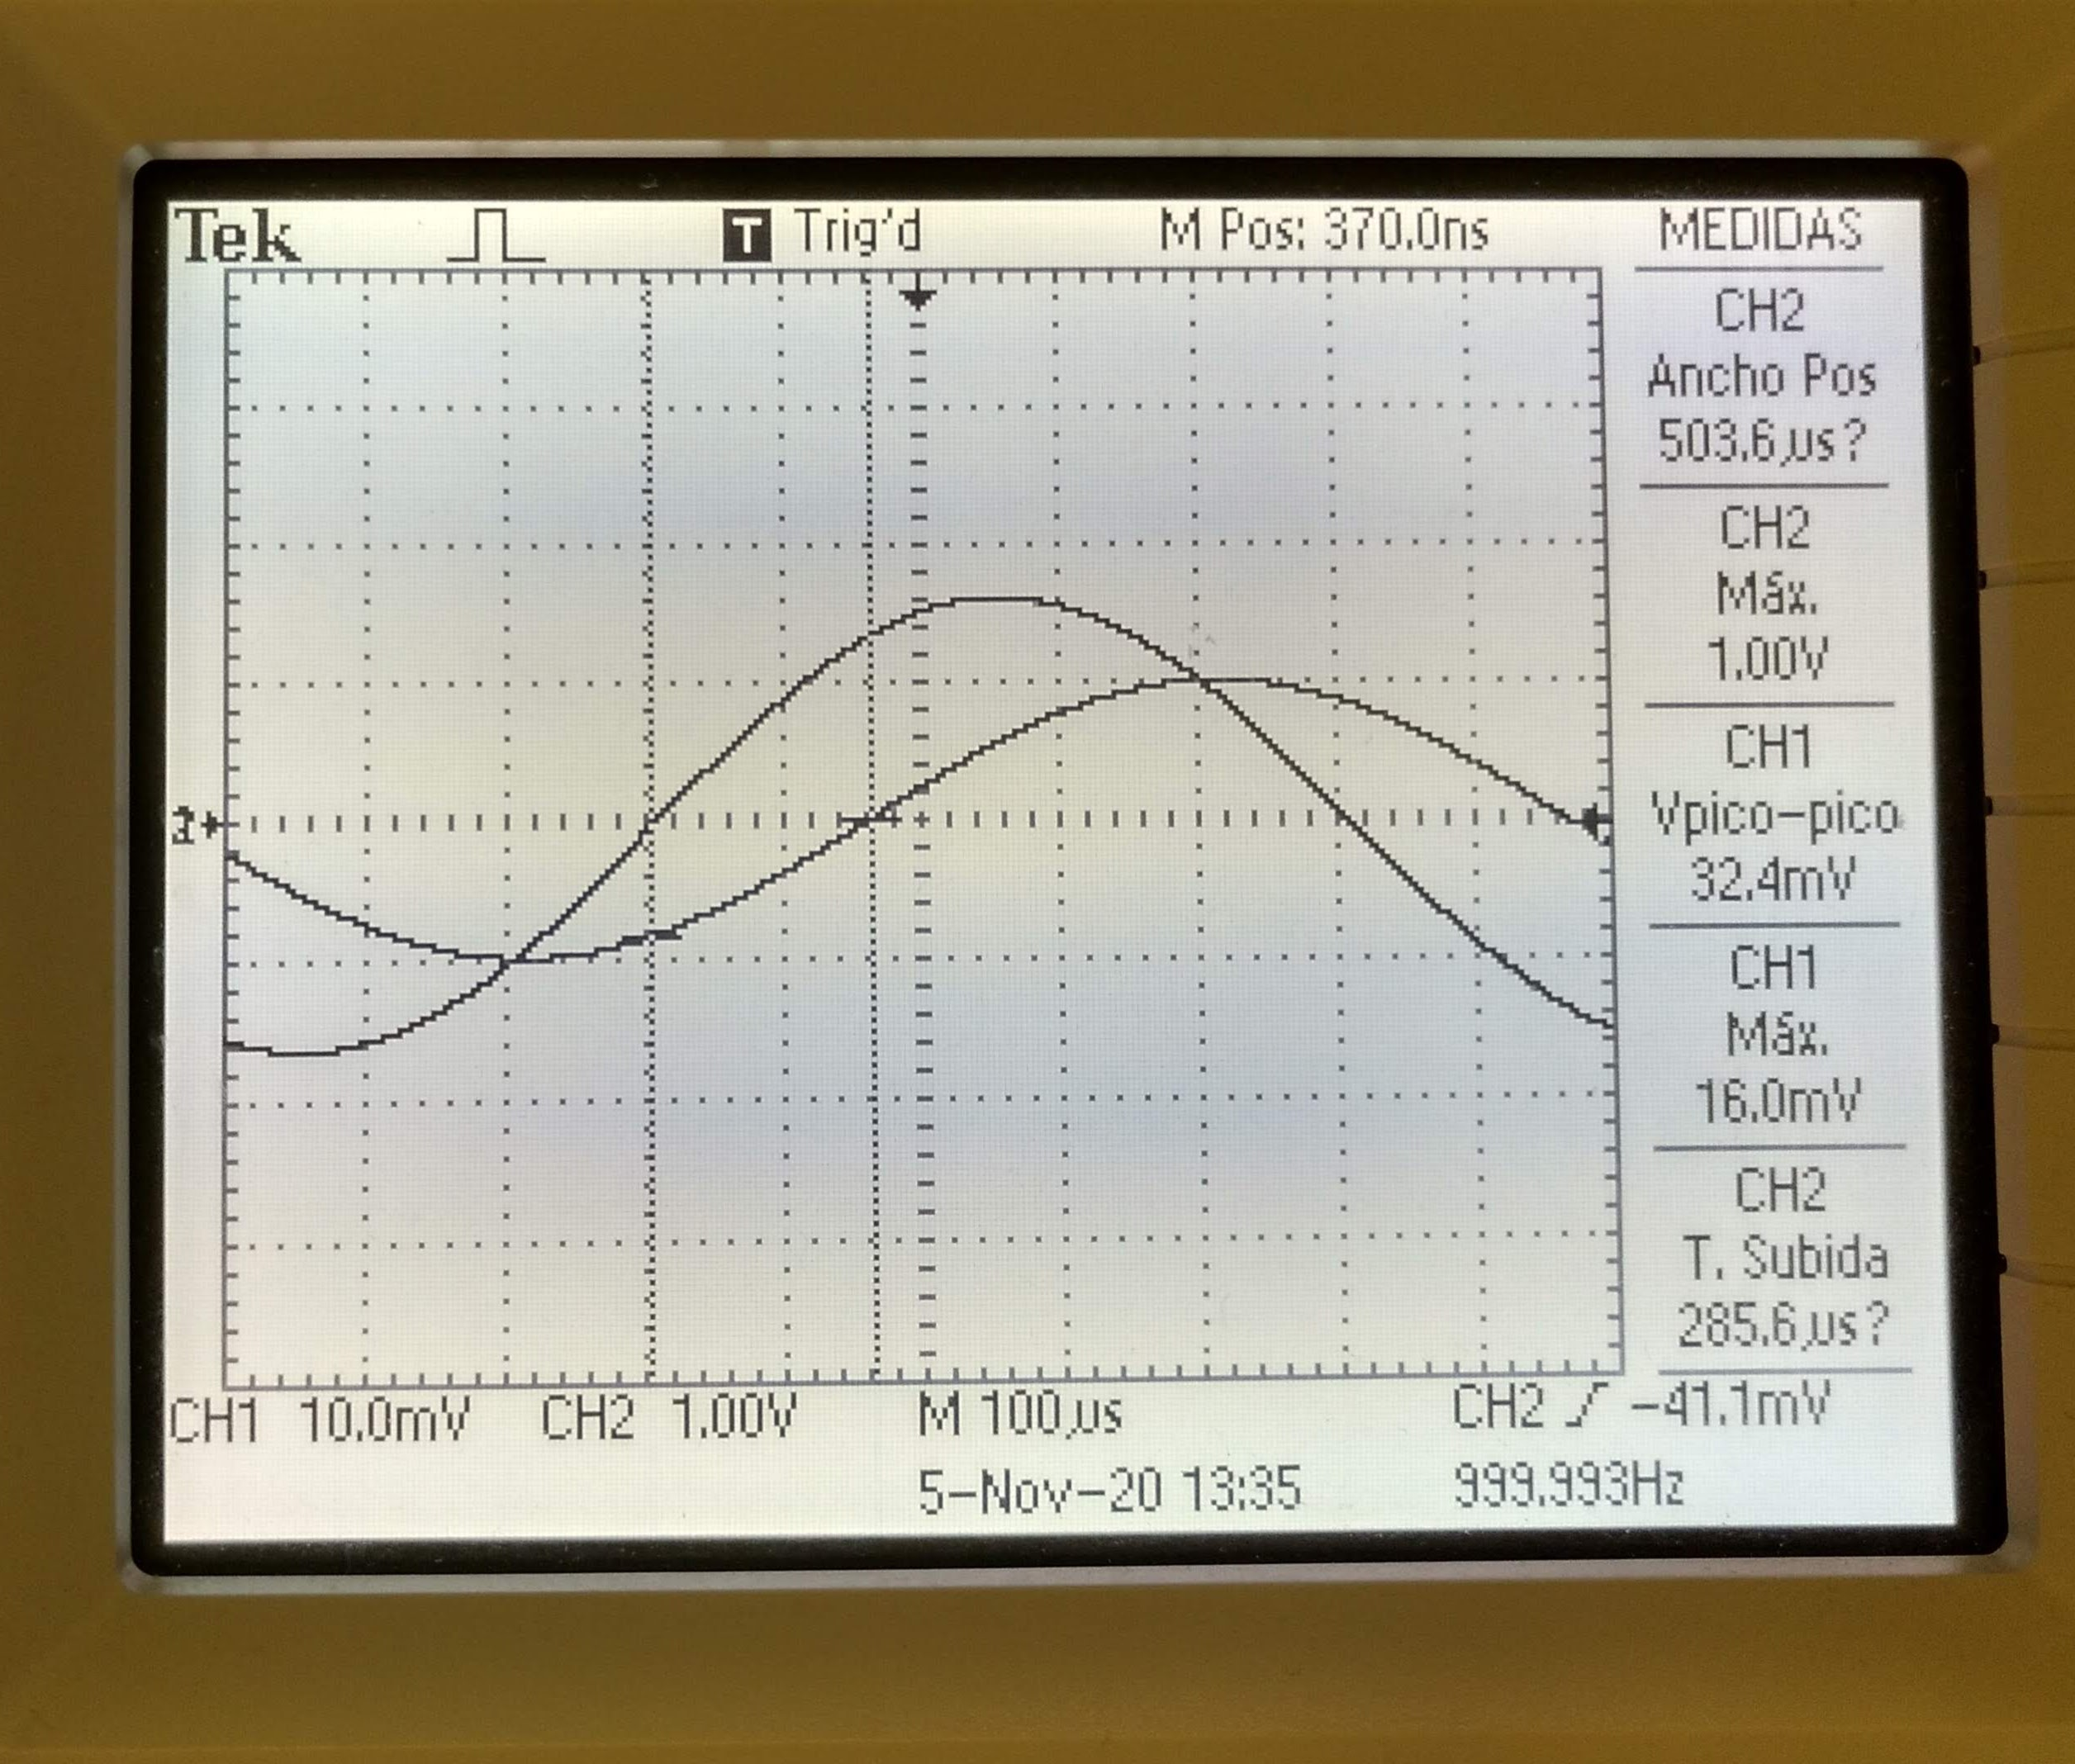
\includegraphics[scale=0.08]{pico} 
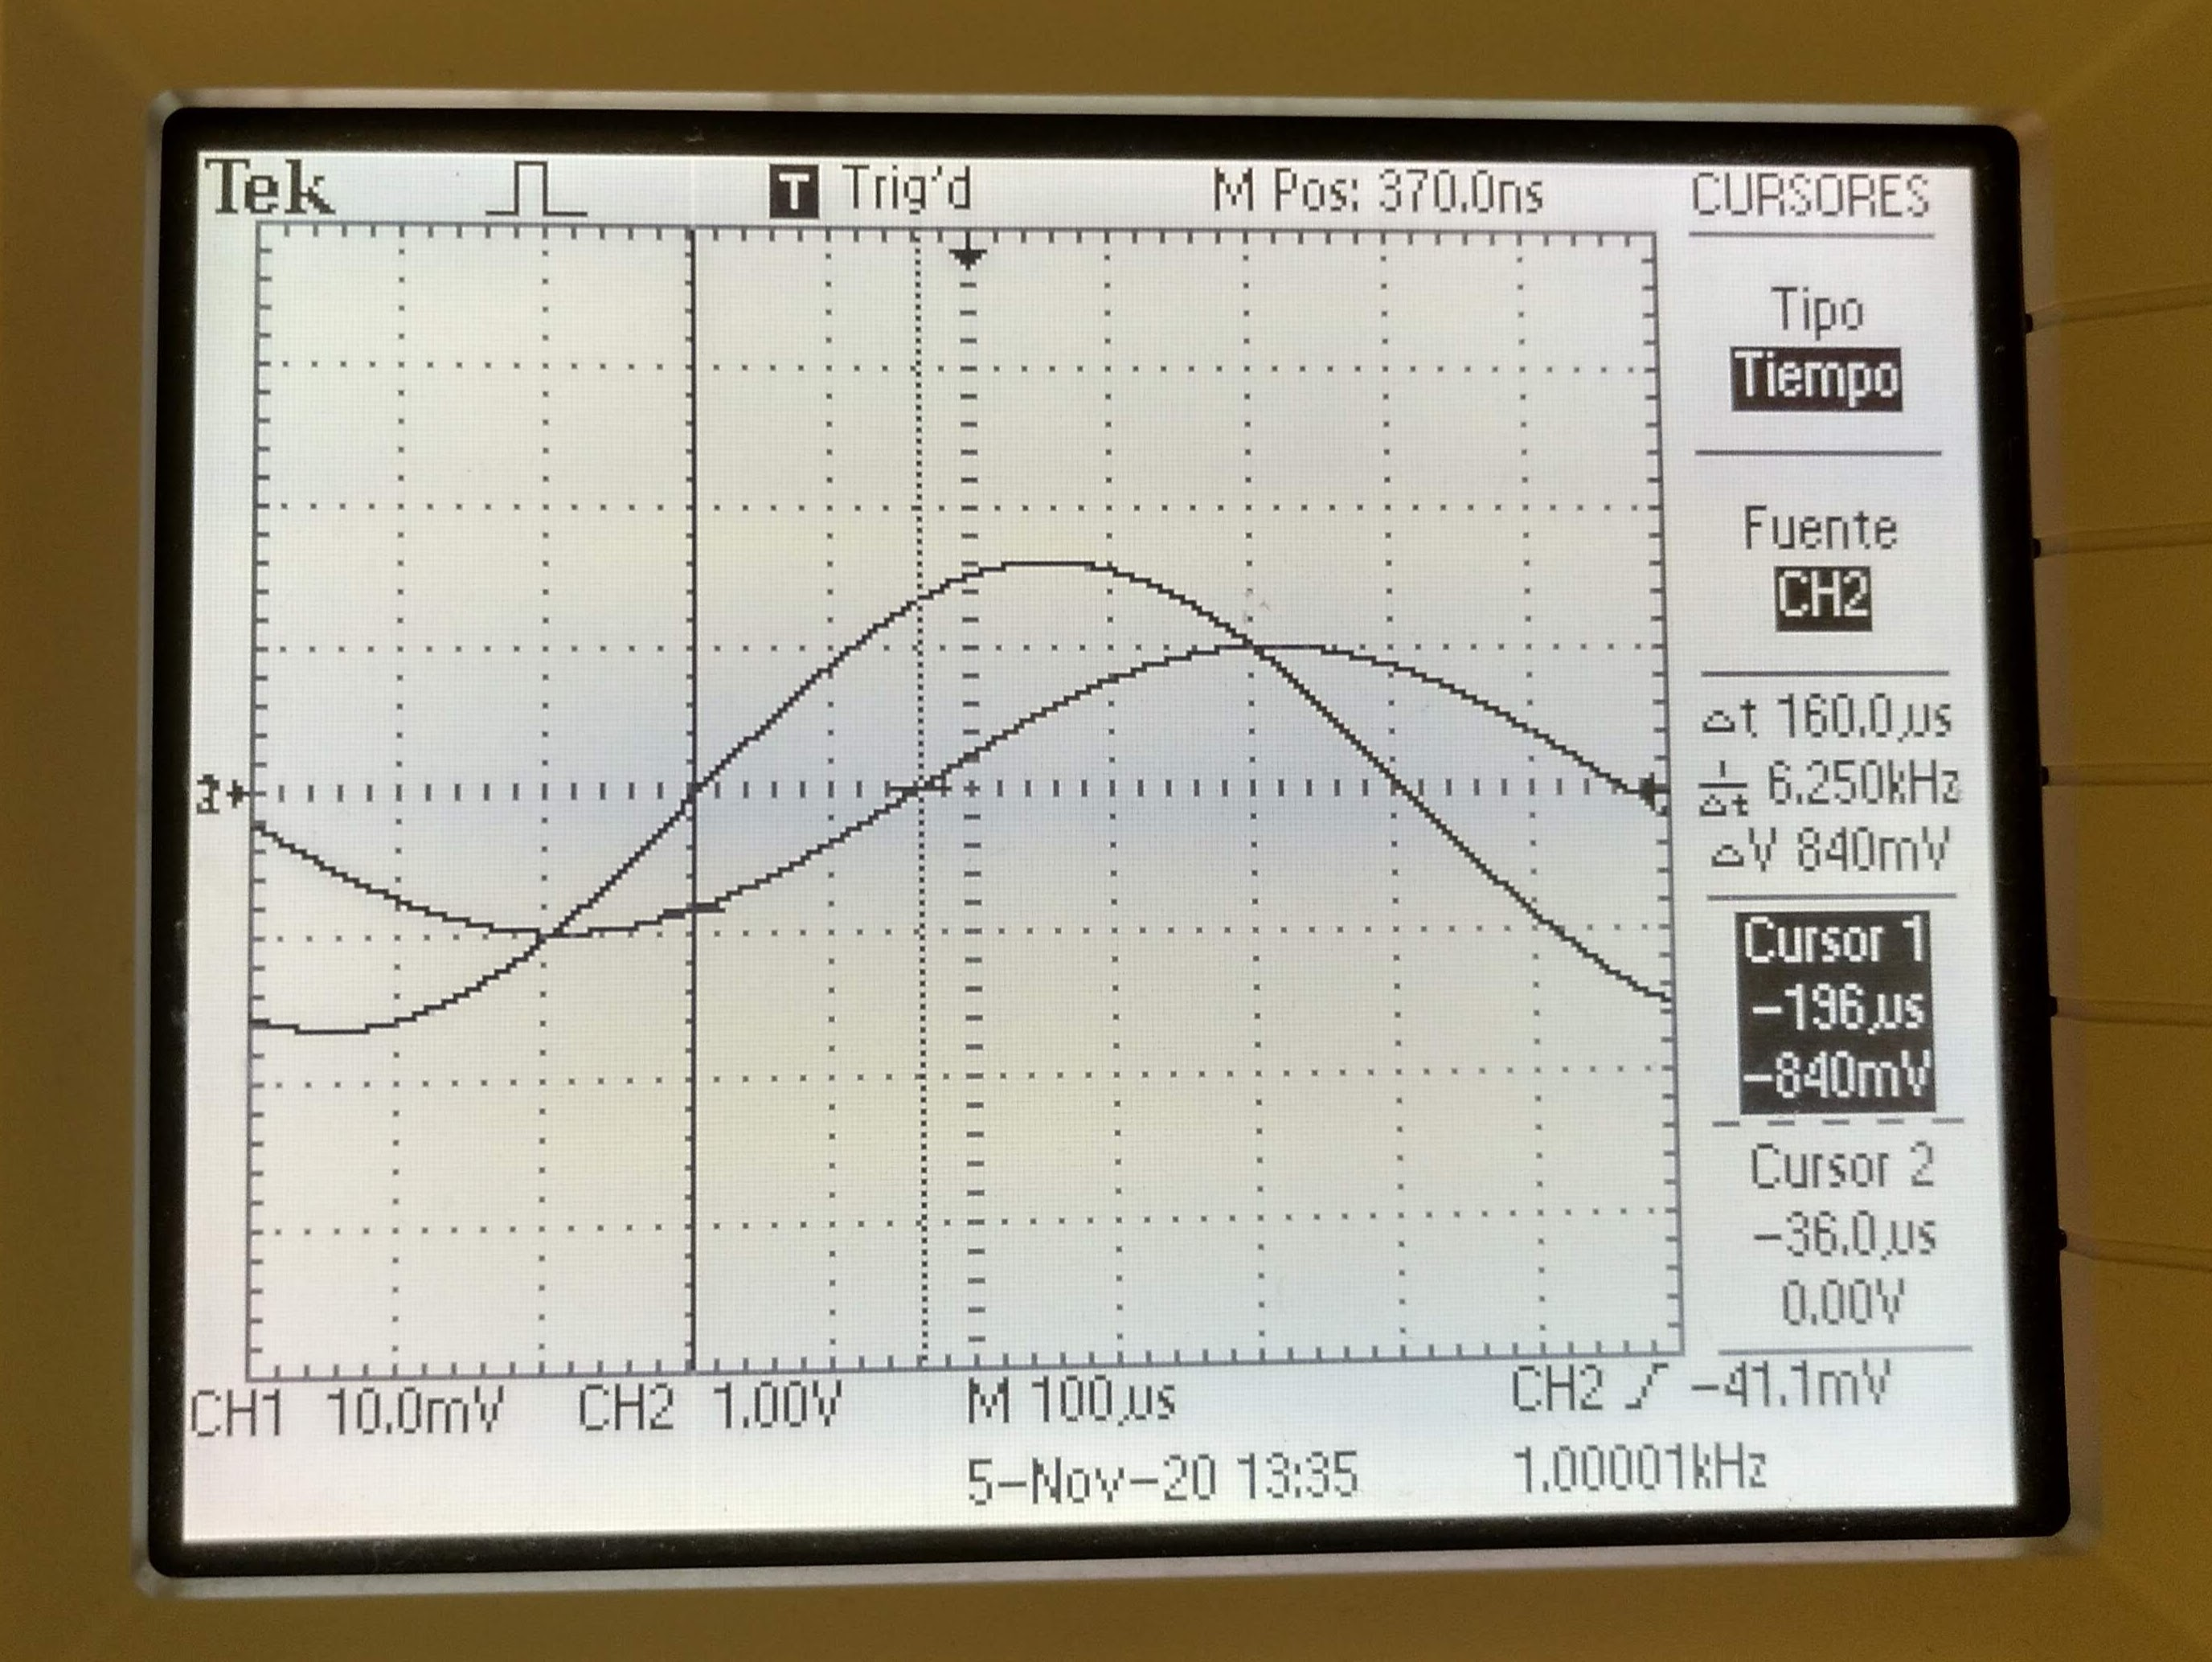
\includegraphics[scale=0.083]{tiem}\\
Ejemplo de la medición del valor Pico-Pico de las ondas (izquierda), y del desfase temporal con los cursores (derecha) en el osciloscopio.
\end{center}

\cleardoublepage
\textbf{Apartado (a)}
Aquí se encuentra la gráfica de los valores experimentales de la ganancia de tensión en decibelios.


\begin{center}
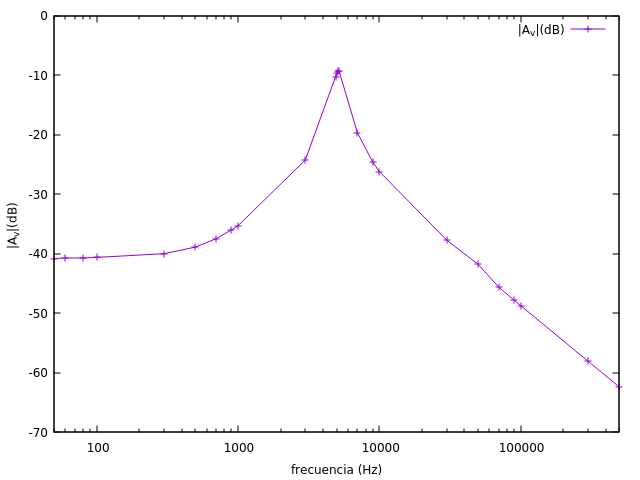
\includegraphics[scale=0.6]{AVdb}\\
\end{center}

Y la gráfica de la diferencia de fase entre $V_1$ y $V_{AB}$:

\begin{center}
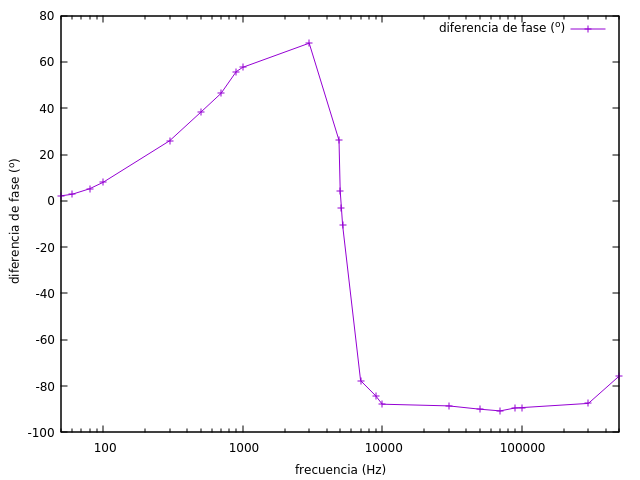
\includegraphics[scale=0.6]{faseg}\\
\end{center}

Ya se comentaron las diferencias entre la simulación con una bobina no (tan) ideal, en la que había una resistencia en serie, la ideal. Por lo que ahora, ya que en el montaje, la bobina tiene una resistencia parásito, vamos a comparar los resultados experimentales con los valores de la simulación de LTSpice, en la que incluimos dicha resistencia. 
\cleardoublepage
\begin{table}[h!]
\centering
\begin{tabular}{|r|r|r|r|r|r|r|}
\hline
\multicolumn{1}{|l|}{frecuencia(Hz)} & \multicolumn{1}{l|}{$A_v$(dB)} & \multicolumn{1}{l|}{LTSpice $A_v$} & \multicolumn{1}{l|}{$E_{absoluto}$ (dB)} & \multicolumn{1}{l|}{$\Phi_1=\Phi (^o)$} & \multicolumn{1}{l|}{$\Phi_2=$LTSpice $\Phi (^o)$} & \multicolumn{1}{l|}{$(\Phi_2 - \Phi_1)(^o)$} \\ \hline
50                                   & -40,82                                              & -44,88                             & 4,06                                     & 2,16                             & 4,416                                    & 2,256                                                                                       \\ \hline
60                                   & -40,72                                              & -44,84                             & 4,12                                     & 2,808                            & 5,256                                    & 2,448                                                                                       \\ \hline
80                                   & -40,71                                              & -44,84                             & 4,13                                     & 5,184                            & 6,99                                     & 1,806                                                                                       \\ \hline
100                                  & -40,62                                              & -44,8                              & 4,18                                     & 7,92                             & 8,75                                     & 0,83                                                                                        \\ \hline
300                                  & -40,00                                              & -44,01                             & 4,01                                     & 25,92                            & 24,58                                    & -1,34                                                                                       \\ \hline
500                                  & -38,88                                              & -42,73                             & 3,85                                     & 38,16                            & 37,23                                    & -0,93                                                                                       \\ \hline
700                                  & -37,50                                              & -41,3                              & 3,80                                     & 46,368                           & 46,32                                    & -0,048                                                                                      \\ \hline
900                                  & -36,00                                              & -39,87                             & 3,87                                     & 55,728                           & 52,9                                     & -2,828                                                                                      \\ \hline
1000                                 & -35,33                                              & -39,17                             & 3,84                                     & 57,6                             & 55,5                                     & -2,1                                                                                        \\ \hline
3000                                 & -24,27                                              & -27,54                             & 3,27                                     & 68,04                            & 69,07                                    & 1,03                                                                                        \\ \hline
5000                                 & -9,66                                               & -11,58                             & 1,92                                     & 4,32                             & 0,877                                    & -3,443                                                                                      \\ \hline
7000                                 & -19,67                                              & -43,38                             & 23,71                                    & -77,616                          & -80,68                                   & -3,064                                                                                      \\ \hline
9000                                 & -24,63                                              & -28,68                             & 4,05                                     & -84,24                           & -86,04                                   & -1,8                                                                                        \\ \hline
10000                                & -26,19                                              & -30,32                             & 4,13                                     & -87,84                           & -87,01                                   & 0,83                                                                                        \\ \hline
30000                                & -37,71                                              & -42,16                             & 4,45                                     & -88,56                           & -89,52                                   & -0,96                                                                                       \\ \hline
50000                                & -41,77                                              & -46,73                             & 4,96                                     & -90                              & -89,73                                   & 0,27                                                                                        \\ \hline
70000                                & -45,60                                              & -49,74                             & 4,14                                     & -90,72                           & -89,81                                   & 0,91                                                                                        \\ \hline
90000                                & -47,79                                              & -51,94                             & 4,15                                     & -89,424                          & -89,85                                   & -0,426                                                                                      \\ \hline
100000                               & -48,69                                              & -52,87                             & 4,18                                     & -89,28                           & -89,87                                   & -0,59                                                                                       \\ \hline
300000                               & -58,04                                              & -62,38                             & 4,34                                     & -87,48                           & -89,96                                   & -2,48                                                                                       \\ \hline
500000                               & -62,38                                              & -66,86                             & 4,48                                     & -75,6                            & -89,97                                   & -14,37                                                                                      \\ \hline
\end{tabular}
\end{table}
Es importante tener en cuenta que la bobina utilizada en el montaje tenía un resistencia en serie parásito de 39,4$\Omega$, mayor que la usada en la simulación del trabajo previo: 40$\Omega$.

Para ver el error de la ganancia, he utilizado el error absoluto, (la diferencia en decibelios), vemos que es aproximadamente 4 en la mayoría de los casos, siendo 23,71dB la mayor diferencia en solamente uno de los casos, con la frecuencia 7000Hz, que posiblemente se deba a un fallo en la medida.

Para el error de los ángulos de la diferencia de fase entre $V_1$ y $V_{AB}$, he recurrido también a la diferencia, con la cual, se aprecia que los desfases medidos en el montaje son muy parecidos a los de la simulación, siendo en todos los casos la diferencia menor de 4$^o$, excepto en la última medida: para 500kHz, la fase difiere en 14,37$^o$ de la fase de la simulación. Cuando la frecuencia tiende a infinito, a las fases deberían acercarse uniformemente a -90$^o$, sin embargo el valor de esta última es mucho mayor que el de las anteriores, posiblemente porque con frecuencias tan altas, es más fácil que se produzcan errores en la medición.
\bigskip

\textbf{Apartado (b)}
El cálculo de la frecuencia natural del filtro es el siguiente: (se calcula el valor de la frecuencia cuando la ganancia es máxima)

$$|A_{v}|(f)=|A_{v}|^{max}=1\iff \left(\omega C - \frac{1}{\omega L}\right)=\left(2\pi fC - \frac{1}{2\pi fL}\right)=0 \iff f=f_0$$

$$f_0=\frac{1}{2\pi \sqrt{CL} }=\frac{1}{2\pi \sqrt{100nF\times10mH} }=5032,92 Hz$$

Una vez calculada esta frecuencia, al tomar los valores experimentales, he medido varias frecuencias cercanas a este valor (como se puede ver en la primera tabla): 4900Hz, 5000Hz, 5100Hz, 5200Hz. De estos valores, el que ha dado una mayor ganancia es el de 5100Hz (esta es entonces la frecuencia natural obtenida experimentalmente). Por tanto, el error relativo del cálculo experimental de la frecuencia natural del circuito es: 
$$E_r=100\times\frac{|f_0-5100Hz|}{f_0}=1,33\%$$

Las frecuencias de corte:

$$\omega=\omega_c\iff |A_v|(\omega)=\frac{1}{\sqrt{1+R_1^2\left(\omega C - \frac{1}{\omega L}\right)^2}}=\frac{1}{\sqrt 2} \iff$$
$$\iff 1=R_1^2\left(\omega C - \frac{1}{\omega L}\right)^2\iff \pm\frac{1}{R_1}=\omega C - \frac{1}{\omega L}\iff 0=\omega^2 CL \mp\frac{\omega L}{R_1} - 1$$

Resolviendo la ecuación de segundo grado:
$$\omega_c=\frac{\pm \frac{ L}{R_1}\pm\sqrt{\frac{ L^2}{R_1^2}+4 CL}}{2CL}=\pm\frac{1}{2CR_1}\pm\sqrt{\frac{1}{4C^2R_1^2}+\frac{1}{CL}}=(\pm 1063,83\pm31640,67)\frac{rad}{s}$$

Y tomando los dos valores positivos (con el segundo término siempre positivo), ya que no tiene sentido una frecuencia negativa:
$$\omega_{CL}=30576,84\frac{rad}{s},\ \ \omega_{CH}=32704,50\frac{rad}{s},\ \ f=\omega /(2\pi)\Longrightarrow f_{CL}=4866,45Hz,\ \  f_{CH}=5205,08Hz$$

Y el ancho de banda el filtro paso banda es entonces: $$\Delta f=f_{CH}-f_{CL}=338,63Hz$$

Ya sabemos, por los datos de la primera tabla, que el máximo valor de la ganancia (según los valores experimentales) es $|A_v|^{max}=|A_v|(5100Hz)\approx 0,3423$, entonces, para las fercuencias de corte, tendremos que $f_{CH}=f_{CL}=|A_v|^{max}/\sqrt 2\approx 0,2420$. Y los valores experimentales que tenemos que más se acercan a esta ganancia son: 4900Hz, por abajo (está debajo de la frecuencia natural, 5100Hz), y por arriba, 5200Hz (conuna diferencia en la ganancia de 0,10). Por tanto, para el caso de la $f_{CL}$, hemos tenido un error de: 
$$E_{r, f_{CL}}=100\times\frac{|f_{CL}-4900Hz|}{f_{CL}}=100\times\frac{|4866,45Hz-4900Hz|}{4866,45Hz}=0,689\%$$
Y para el caso de la $f_{CH}$, (tenemos que $|A_v|(5200Hz)=0,34$ y $|A_v|(7000Hz)=0,10$, por lo que ambos están lejos de el valor de $|A_v|(f_{CH})\approx 0,24$, aunque con 5200Hz nos acercamos más en cuanto a la ganancia):
$$E_{r, f_{CH}}=100\times\frac{|f_{CH}-5200Hz|}{f_{CH}}=100\times\frac{|5205,08Hz-5200Hz|}{5205,08Hz}=0,098\%$$
Aunque este error es muy bajo, se ha hecho tomando el valor más cercano posible (de entre los medidos), pero había una diferencia entre la ganancia de esta frecuencia medida, 5200Hz y la supuesta ganancia en la frecuencia de corte $|A_v|^{max}/\sqrt 2\approx 0,2420$ de 0,1. Por lo que habríamos sido más precisos si hubiéramos tomado medidas en frecuencias un poco mayores de 5200Hz para haber sido más exactos.

\bigskip

\textbf{A continuación, mediremos la amplitud de los armónicos de una señal cuadrada en V1
utilizando el filtro paso banda. Como no podemos incrementar la frecuencia central del filtro
de forma continua con los componentes disponibles, mediremos la amplitud a la salida a medida
que disminuimos la frecuencia de V1 progresivamente.}

\textbf{Utilizando el mismo montaje de la 1ª parte, seleccione una señal alterna de forma
cuadrada para V1.}

\textbf{Fije la frecuencia de la onda cuadrada en el valor de la frecuencia central del filtro. Mida
la amplitud de la onda V1 ($V_1$) y la amplitud de la onda entre A y B ($V_{AB}$).}

\textbf{Fije la frecuencia de la onda cuadrada en el valor de la frecuencia central del filtro
dividido por tres. En ese momento se observa un aumento de la amplitud de la onda de salida
debido al filtrado selectivo del armónico de orden 3. Mida la amplitud de la onda V1 ($V_1$) y la
amplitud de la onda entre A y B ($V_{AB}$).}

\textbf{Fije la frecuencia de la onda cuadrada en el valor de la frecuencia central del filtro
dividido por k. En ese momento se observa un aumento de la amplitud de la onda de salida
debido al filtrado del armónico selectivo de orden k. Mida la amplitud de la onda V1 ($V_1$) y la
amplitud de la onda entre A y B ($V_{AB}$).}

\textbf{Repita las medidas hasta que la onda de salida se confunda con el ruido del sistema.}

\textbf{c) Con los datos medidos se debería poder rellenar una tabla como la siguiente:}
\bigskip

Para rellenar la tabla (en concreto la columna en la que se representa $4/(\pi k) A_{v}^{max}$), he utilizado el valor de $A_{v}^{max}=0,3423$, el cual es el valor máximo medido experimentalmente para la ganancia (con $f=5100Hz$).

\begin{table}[h]
\centering
\begin{tabular}{|r|r|r|r|r|r|r|}
\hline
\multicolumn{1}{|l|}{orden ($k$)} & \multicolumn{1}{l|}{f(V1) (Hz)=$f_0/k$} & \multicolumn{1}{l|}{$V_1(V)$} & \multicolumn{1}{l|}{$V_{AB}(V)$} & \multicolumn{1}{l|}{$A_v$} & \multicolumn{1}{l|}{$4/(\pi k) A_{v}^{max}$} & \multicolumn{1}{l|}{ERROR (\%)} \\ \hline
1                                            & 5100                                            & 1,04                          & 0,48                             & 0,4615384615               & 0,4358396903                                 & 5,896381582                     \\ \hline
3                                            & 1700                                            & 1,02                          & 0,23                             & 0,2254901961               & 0,1452798968                                 & 55,210873                       \\ \hline
5                                            & 1020                                            & 1                             & 0,17                             & 0,17                       & 0,08716793806                                & 95,02583608                     \\ \hline
7                                            & 728,5714286                                     & 1,02                          & 0,14                             & 0,137254902                & 0,0622628129                                 & 120,4444283                     \\ \hline
9                                            & 566,6666667                                     & 1,02                          & 0,132                            & 0,1294117647               & 0,04842663226                                & 167,2326335                     \\ \hline
11                                           & 463,6363636                                     & 1,02                          & 0,128                            & 0,1254901961               & 0,03962179003                                & 216,7201582                     \\ \hline
13                                           & 392,3076923                                     & 1,02                          & 0,126                            & 0,1235294118               & 0,03352613002                                & 268,4571159                     \\ \hline
15                                           & 340                                             & 1,02                          & 0,102                            & 0,1                        & 0,02905597935                                & 244,1632401                     \\ \hline
17                                           & 300                                             & 1,04                          & 0,1                              & 0,09615384615              & 0,02563762884                                & 275,0496848                     \\ \hline
19                                           & 268,4210526                                     & 1,04                          & 0,1                              & 0,09615384615              & 0,02293893107                                & 319,1731771                     \\ \hline
\end{tabular}
\end{table}

Como se ve en la tabla, los errores son muy altos: mayores del $50\%$, a partir del armónico de orden 3; aunque el armónico de orden 1 se ha medido con un error de únicamente $5,89\%$. 
Estos errores son causados por la limitación de tener que ir variando la frecuencia de entrada, ya que no podemos aumentar la frecuencia central de nuestro circuito de forma continua. Esto causa que tengamos que hacer mediciones con frecuencias cada vez más bajas, con mucho ruido y por tanto muy imprecisas. Llega un punto en que por mucho que se baje la frecuencia (aumentando el orden del armónico), todos dan un mismo valor, aunque las frecuencias no se parezcan tanto, y las ondas no tienen forma sinusoidal.
\bigskip
\begin{center}
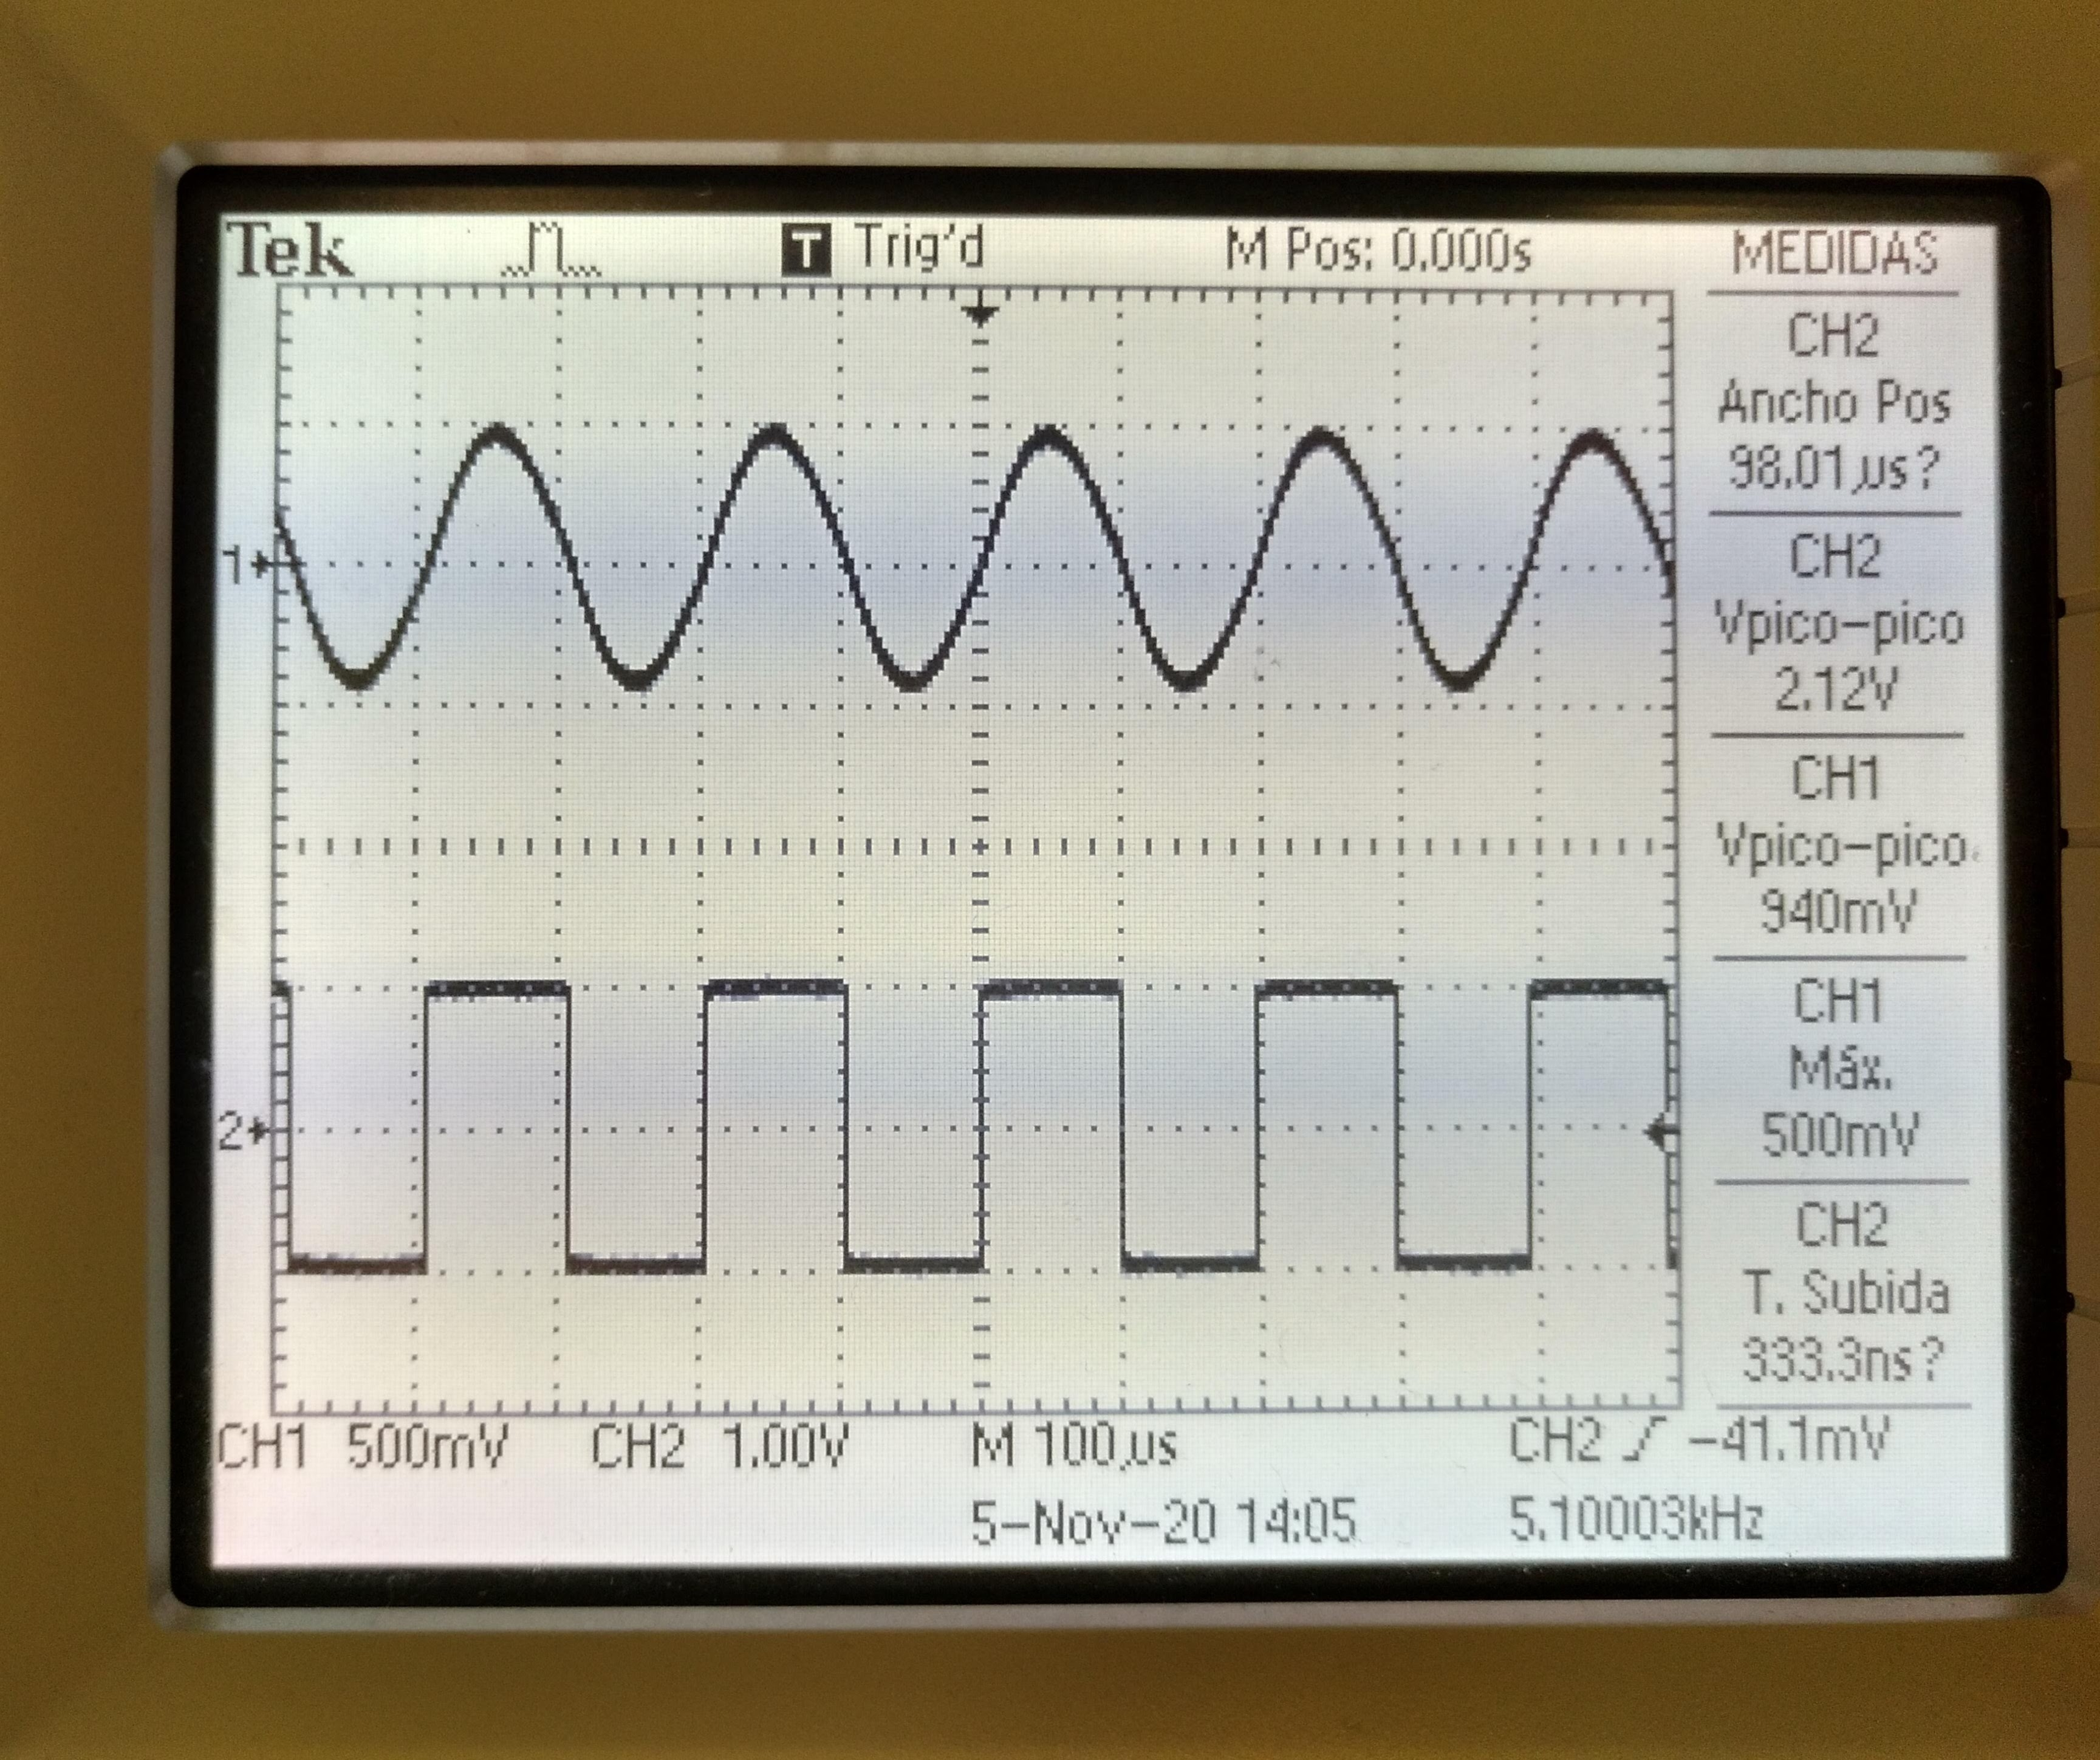
\includegraphics[scale=0.075]{ondas}\\
Ejemplo de cómo se han medido en el osciloscopio los valores pico-pico para cada frecuencia.
\end{center}

\textbf{Apartado (d)}
En esta práctica hemos observado la gran cantidad de desviaciones que causa el trabajar teóricamente con filtros ideales. En particular, el cambio en los resultados que supone el tener una bobina ideal, o una con una resistencia parásito (más parecida a la real). Aún así, se han producido grandes desviaciones en los valores experimentales y los simulados con esta resistencia parásito, aunque las gráficas obtenidas del montaje sí que se parecen a lo esperado (en cuanto a las asintotas - un \textit{plateau} en los $\sim -40dB$ para frecuencias bajas - y los máximos). Por tanto, lo más seguro es que los errores que se hayan producido se deban principalmente a que la resistencia que hemos usado no era exactamente de 4,70k$\Omega$, sino de 4,64k$\Omega$, y a las variaciones en los valores del condensador y la bobina, que tenía también unos valores un poco distintos, como ya se ha comentado anteriormente. De todos modos, el valor de la frecuencia natural del filtro apenas se ha desviado de lo esperado teóricamente, siendo el valor que más se ha acercado tanto en la simulación como en el montaje. 



\end{document}